% ECE 442 / CSC 402 Progress Report
% Don Nguyen

\documentclass[11pt]{article}

\usepackage[top=0.75in, bottom=0.75in, left=0.75in, right=0.75in]{geometry}
\usepackage{amsmath,amsfonts,amssymb}
\usepackage{graphicx}
\usepackage{hyperref}
\usepackage{url}
\usepackage{enumitem}
\usepackage{booktabs}
\usepackage{algorithm}
\usepackage{algpseudocode}

\title{
Agentic Relational Reasoning with Knowledge Graph Memory \\
for Enterprise Databases \\
\large Progress Report
}

\author{
  Don Nguyen \\
  CSC 402 / ECE 442 -- Network Science Analytics \\
  University of Rochester \\
  \texttt{knguy42@u.rochester.edu}
}

\begin{document}

\maketitle

\begin{abstract}
This progress report describes work completed toward building a knowledge graph memory layer for enterprise database querying agents, targeting the Spider~2.0 and BIRD benchmarks.
Since the proposal, we have finalized the heterogeneous information network (HIN) schema, formally defined the graph model and retrieval algorithm, deployed a live graph database instance (Neo4j Aura), and bootstrapped the graph with schema metadata from all BIRD databases and a sponsored Spider~2.0 Snowflake warehouse.
Obtaining programmatic access to the Spider~2.0 Snowflake instance---identified as a key infrastructure risk in the proposal---has been resolved.
The graph currently contains 107 database nodes, 9{,}093 table nodes, 56{,}939 column nodes, and 91 foreign-key edges ingested so far, with ingestion still in progress.
We describe the formal graph model, construction methodology, agent architecture, complications encountered, and remaining work.
\end{abstract}

% -----------------------------------------------------------------------
\section{Introduction and Problem Statement}
% -----------------------------------------------------------------------

Large language models (LLMs) have demonstrated strong performance on text-to-SQL benchmarks, yet they still fail on the most complex real-world database tasks.
Two fundamental bottlenecks explain this gap.
First, \emph{context window saturation}: enterprise databases routinely have 50--200+ tables with thousands of columns, far exceeding what can be injected into an LLM context at once.
Second, \emph{loss of relational structure}: standard retrieval systems treat schema elements as flat text, discarding the network topology---foreign-key paths, join graphs, entity hierarchies---that is essential for multi-hop SQL reasoning.

The Spider~2.0 benchmark~\cite{yu2024spider2} was specifically designed to expose these failures, featuring complex enterprise workflows across large Snowflake and BigQuery schemas where state-of-the-art models achieve below 20\% success.
Similarly, the BIRD benchmark~\cite{li2024bird} requires agents to navigate multi-turn dialogs over large, realistic databases.

The severity of this failure is quantified by the benchmarks themselves.
On Spider~2.0, the best published agents achieve only 17--19\% success rate~\cite{yu2024spider2}.
On BIRD, top models reach approximately 60\% execution accuracy~\cite{li2024bird}, but performance degrades sharply on the hardest multi-hop questions.
These numbers set the baseline our system aims to improve upon.

\textbf{Problem statement.}
We aim to build and evaluate a \emph{knowledge graph memory layer} for text-to-SQL agents.
The graph is a heterogeneous information network (HIN) constructed from database schemas, documentation, and business logic definitions.
An agent equipped with graph navigation tools can retrieve only the relevant schema neighborhood for each question, rather than being overwhelmed by the full schema.
We evaluate whether this graph-based memory improves execution accuracy on BIRD and Spider~2.0 compared to baselines that do not use structured graph context.

% -----------------------------------------------------------------------
\section{Literature Review}
% -----------------------------------------------------------------------

\paragraph{Text-to-SQL benchmarks.}
The original Spider benchmark~\cite{yu2018spider} introduced cross-domain text-to-SQL evaluation.
Spider~2.0~\cite{yu2024spider2} significantly raises the difficulty by targeting enterprise-scale schemas hosted on cloud data warehouses (Snowflake, BigQuery), requiring agents to handle 1{,}000+ column schemas, multi-step workflows, and external business knowledge.
BIRD~\cite{li2024bird} focuses on conversational, multi-turn SQL reasoning where agents must maintain context across turns---a natural setting for persistent graph memory.

\paragraph{Schema linking and pruning.}
DIN-SQL~\cite{pourreza2023dinsql} decomposes text-to-SQL into sub-problems including schema linking, but operates entirely on flat text.
DAIL-SQL~\cite{gao2023dailsql} selects relevant schema elements via similarity search, again without exploiting relational graph structure.
Both achieve strong results on simpler benchmarks but degrade sharply when schemas grow large.

\paragraph{Graph-structured representations.}
Heterogeneous information networks (HINs)~\cite{sun2013survey} provide a principled framework for modeling multi-typed entities and relations.
Relational graph convolutional networks (R-GCNs)~\cite{schlichtkrull2018rgcn} demonstrate that graph neural network message passing over typed edges can learn rich relational representations.
More recently, Fey et al.~\cite{fey2023relbench} propose relational deep learning over database graphs, treating the entire database as a graph for representation learning.
Our work differs in that we use the graph as an \emph{agent memory and retrieval layer} rather than as input to a learned model---a distinction that allows us to leverage existing LLMs without retraining.

\paragraph{Agentic SQL systems.}
Recent work on agentic text-to-SQL~\cite{yu2024spider2} uses LLMs with tool-calling to iteratively explore schemas, but without persistent structured memory.
LangGraph~\cite{langgraph} provides an orchestration framework for stateful multi-step agent workflows, which we adopt for our agent loop.

% -----------------------------------------------------------------------
\section{Methods}
% -----------------------------------------------------------------------

\subsection{Formal Graph Model}

We define the knowledge graph as a typed heterogeneous information network:

\[
G = (V,\, E,\, \phi : V \to \mathcal{T}_V,\, \psi : E \to \mathcal{T}_E)
\]

where $V$ is the set of nodes, $E \subseteq V \times V$ is the set of directed edges, $\phi$ maps each node to one of five types $\mathcal{T}_V = \{\texttt{Database},\allowbreak\texttt{Table},\allowbreak\texttt{Column},\allowbreak\texttt{Metric},\allowbreak\texttt{DbtModel}\}$, and $\psi$ maps each edge to one of seven types $\mathcal{T}_E = \{\texttt{HAS},\allowbreak\texttt{FK},\allowbreak\texttt{REFERENCES},\allowbreak\texttt{DEPENDS\_ON},\allowbreak\texttt{READS},\allowbreak\texttt{PRODUCES}\}$.

Each node $v \in V$ carries a property vector $\mathbf{p}(v)$ encoding structured metadata (e.g., column data type, nullability, sample values).
The \texttt{FK} edges form a foreign-key subgraph $G_{\text{FK}} = (V_C, E_{\text{FK}})$ over the column nodes $V_C = \phi^{-1}(\texttt{Column})$, which is the primary structure used for join path discovery.

\subsection{Graph-Guided Schema Retrieval}

The key operation during agent inference is \emph{relevant subgraph extraction}.
Given a natural-language question $q$ and a database $d$, the agent must identify a small subgraph $G_q \subset G$ containing the tables and columns needed to answer $q$.
We implement this via a sequence of Cypher-backed tool calls.

The most critical tool is join path discovery.
Given two table names $t_a, t_b$ in database $d$, we find the shortest path in $G_{\text{FK}}$ between any column of $t_a$ and any column of $t_b$:

\[
\texttt{find\_join\_path}(d, t_a, t_b) = \arg\min_{\pi} |\pi|
\]

where $\pi$ is a path in $G_{\text{FK}}$ from $\phi^{-1}(t_a)$ to $\phi^{-1}(t_b)$.
This is implemented as a bounded-depth Cypher shortest-path query:

\begin{verbatim}
MATCH p = shortestPath(
  (a:Column {db_id:$db, table_name:$ta})
  -[:FK*1..6]->
  (b:Column {db_id:$db, table_name:$tb}))
RETURN p
\end{verbatim}

The full tool API exposed to the agent is:

\begin{itemize}[leftmargin=*]
  \item \texttt{get\_tables(db\_id)} $\to$ table names and descriptions.
  \item \texttt{get\_columns(db\_id, table\_name)} $\to$ column metadata and sample values.
  \item \texttt{find\_join\_path(db\_id, table\_a, table\_b)} $\to$ shortest FK path.
  \item \texttt{search\_columns(db\_id, keyword)} $\to$ columns matching a keyword.
  \item \texttt{get\_metric(db\_id, metric\_name)} $\to$ business metric definition.
  \item \texttt{get\_dbt\_lineage(db\_id, model\_name)} $\to$ dbt model dependencies.
\end{itemize}

\subsection{Graph Construction Algorithm}

Algorithm~\ref{alg:bootstrap} describes the schema ingestion procedure for a single database.
All writes use idempotent \texttt{MERGE} operations so the procedure is safely restartable.

\begin{algorithm}
\caption{Schema bootstrap for database $d$}
\label{alg:bootstrap}
\begin{algorithmic}[1]
\Require Database connection $\mathcal{D}$, Neo4j driver $\mathcal{N}$, database id $d$
\State \textbf{MERGE} $(\texttt{Database}\{db\_id: d\})$ into $\mathcal{N}$
\For{each table $t$ in $\mathcal{D}.\texttt{INFORMATION\_SCHEMA.TABLES}$}
  \State \textbf{MERGE} $(\texttt{Table}\{db\_id: d, name: t\})$ into $\mathcal{N}$
  \State \textbf{MERGE} $(\texttt{Database}\ d) \xrightarrow{\texttt{HAS}} (\texttt{Table}\ t)$
  \For{each column $c$ in $t$}
    \State \textbf{MERGE} $(\texttt{Column}\{db\_id: d, table: t, name: c\})$ into $\mathcal{N}$
    \State \textbf{MERGE} $(\texttt{Table}\ t) \xrightarrow{\texttt{HAS}} (\texttt{Column}\ c)$
  \EndFor
\EndFor
\For{each FK constraint $(c_{\text{src}}, c_{\text{dst}})$ in $\mathcal{D}$}
  \State \textbf{MERGE} $(\texttt{Column}\ c_{\text{src}}) \xrightarrow{\texttt{FK}} (\texttt{Column}\ c_{\text{dst}})$
\EndFor
\end{algorithmic}
\end{algorithm}

\subsection{Agent Architecture}

The agent is a directed cyclic graph implemented in LangGraph with four node types:

\begin{enumerate}[leftmargin=*]
  \item \textbf{Graph retrieval}: the LLM issues 2--4 tool calls against Neo4j to retrieve a relevant schema subgraph $G_q$.
  \item \textbf{SQL generation}: $G_q$ is serialized into a compact text representation and provided to the LLM (Nemotron via NVIDIA NIM) to generate candidate SQL.
  \item \textbf{SQL execution}: the candidate query is executed against the target database (Snowflake for Spider~2.0, SQLite for BIRD). Results and any error messages are captured.
  \item \textbf{Self-correction}: on error or unexpected output, execution feedback is returned to step 1, allowing the agent to issue additional graph queries and revise the SQL. A maximum retry depth is enforced.
\end{enumerate}

The key design principle is that the agent \emph{never} receives the full database schema. Instead, it navigates the graph to assemble a minimal context window containing only the relevant tables, columns, join paths, and business definitions.

% -----------------------------------------------------------------------
\section{Data Collection and Network Construction}
% -----------------------------------------------------------------------

\subsection{Data Sources}

We use two benchmark suites:

\begin{itemize}[leftmargin=*]
  \item \textbf{BIRD}~\cite{li2024bird}: 80 databases (69 training + 11 validation). Schemas are provided as SQLite files and a \texttt{train\_tables.json} manifest. External knowledge is provided per-database as Markdown files.
  \item \textbf{Spider~2.0}~\cite{yu2024spider2}: 114 databases used across benchmark tasks, hosted on a sponsored Snowflake instance. Schemas are introspected via \texttt{INFORMATION\_SCHEMA}. Only the 114 task-relevant databases are ingested (filtered from the 155-database Snowflake account).
\end{itemize}

\subsection{HIN Schema and Visualization}

Figure~\ref{fig:hin} illustrates the HIN node and edge types.

\begin{figure}[h]
\centering
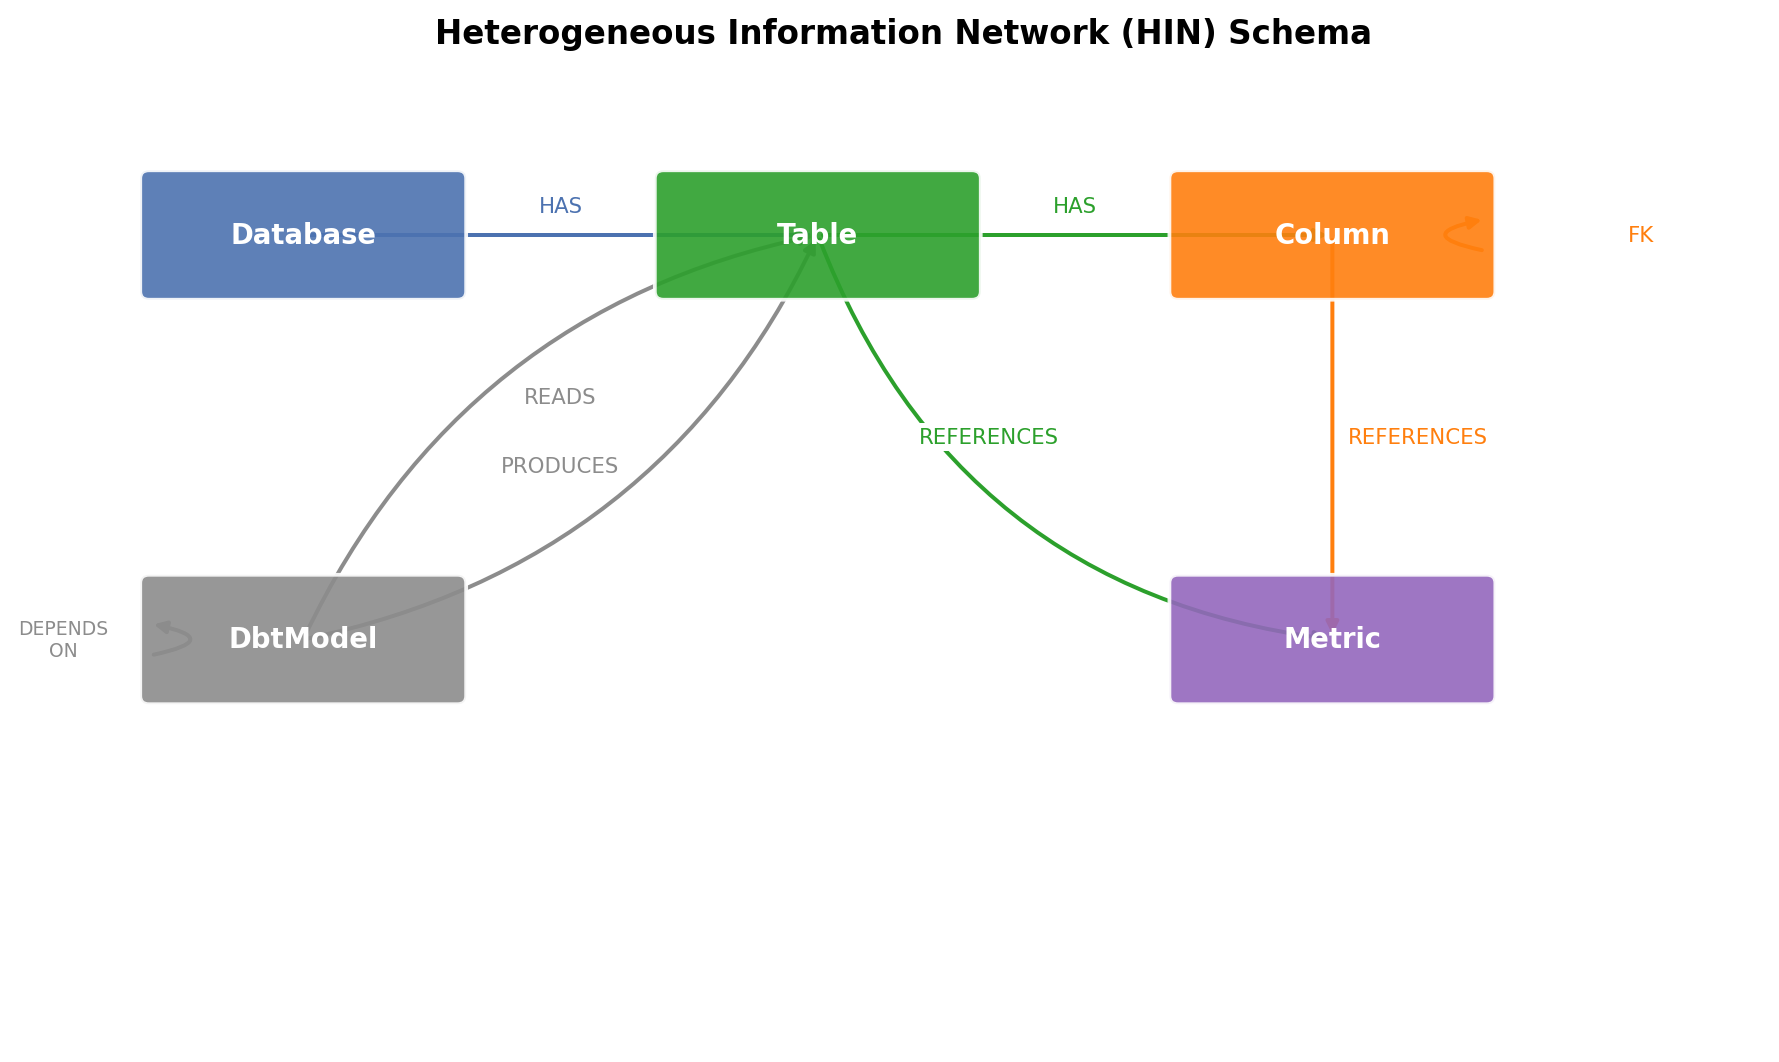
\includegraphics[width=0.88\textwidth]{hin_diagram.png}
\caption{Heterogeneous Information Network schema. Node colors denote type; edges encode structural (\texttt{HAS}, \texttt{FK}), semantic (\texttt{REFERENCES}), and lineage (\texttt{READS}, \texttt{PRODUCES}, \texttt{DEPENDS\_ON}) relationships.}
\label{fig:hin}
\end{figure}

\subsection{Bootstrap Implementation}

Two bootstrap scripts populate Neo4j:

\begin{enumerate}[leftmargin=*]
  \item \textbf{BIRD bootstrap}: parses \texttt{train\_tables.json} and introspects SQLite files via \texttt{PRAGMA table\_info} and \texttt{PRAGMA foreign\_key\_list}.
  \item \textbf{Spider~2.0 Snowflake bootstrap}: connects to the Snowflake instance via TOTP-authenticated programmatic access and queries \texttt{INFORMATION\_SCHEMA} per database. The script filters to only the 114 task-relevant databases and is designed for resumability---already-ingested databases are detected at startup and skipped.
\end{enumerate}

% -----------------------------------------------------------------------
\section{Preliminary Results}
% -----------------------------------------------------------------------

\subsection{Graph Population Progress}

Table~\ref{tab:status} summarizes the current implementation status.
The graph currently contains the following nodes and edges (as of report submission, with Spider~2.0 ingestion still in progress):

\begin{center}
\begin{tabular}{lr}
\toprule
\textbf{Node / Edge type} & \textbf{Count} \\
\midrule
Database nodes (total) & 107 \\
\quad BIRD databases & 16 \\
\quad Spider~2.0 databases & 91 \\
Table nodes & 9{,}093 \\
Column nodes & 56{,}939 \\
FK edges & 91 \\
\bottomrule
\end{tabular}
\end{center}

The low FK edge count (91 across 9{,}093 tables) reflects the well-known fact that analytical data warehouses rarely declare formal referential constraints.
This motivates our planned heuristic FK inference step, which will match column names across tables within the same database (e.g., a column named \texttt{customer\_id} in two different tables implies a likely join relationship).

\begin{table}[h]
\centering
\begin{tabular}{lll}
\toprule
\textbf{Component} & \textbf{Status} & \textbf{Notes} \\
\midrule
HIN schema design        & Complete     & 5 node types, 7 edge types \\
Formal graph model       & Complete     & HIN definition, FK path formalization \\
Neo4j Aura instance      & Complete     & Live, connected \\
BIRD schema bootstrap    & Complete     & 80 databases ingested \\
Snowflake access         & Complete     & Major risk resolved \\
Spider~2.0 bootstrap     & In progress  & 91/114 task databases ingested \\
Graph tool API           & In progress  & Design complete, implementation pending \\
LangGraph agent          & In progress  & Architecture designed \\
Inferred FK edges        & Not started  & Column-name heuristic planned \\
Metric node ingestion    & Not started  & From Spider~2.0 external knowledge docs \\
Baseline evaluation      & Not started  & Planned next \\
\bottomrule
\end{tabular}
\caption{Component status as of progress report submission.}
\label{tab:status}
\end{table}

\subsection{Schema Complexity and Graph Structure}

Figure~\ref{fig:graphstats} shows the distribution of tables per database and columns per table across the Spider~2.0 databases ingested so far.
Both distributions are highly right-skewed (plotted on log axes), with the following statistics from the live Neo4j graph:

\begin{itemize}[leftmargin=*]
  \item \textbf{Columns per table}: min 1, max 1{,}148, median 9, mean 26.9. The heavy tail is driven by large scientific schemas (e.g., \texttt{EBI\_CHEMBL} with 785 tables).
  \item \textbf{Tables per database}: min 1, max 4{,}989, median 8. The largest database (\texttt{GITHUB\_REPOS\_DATE}) has nearly 5{,}000 tables---completely infeasible to inject into any LLM context.
  \item \textbf{FK sparsity}: only 91 FK edges across 9{,}093 tables (less than 0.01 FK per table on average). The declared FK subgraph $G_{\text{FK}}$ is nearly empty, meaning join path discovery via declared constraints alone is infeasible. Heuristic FK inference is not optional---it is the primary mechanism for join path discovery in this benchmark.
\end{itemize}

These structural properties of the benchmark directly validate the graph-based approach: flat schema injection is impossible for the largest databases, and the near-absence of FK constraints means the agent cannot rely on the database schema alone to discover join paths.

\begin{figure}[h]
\centering
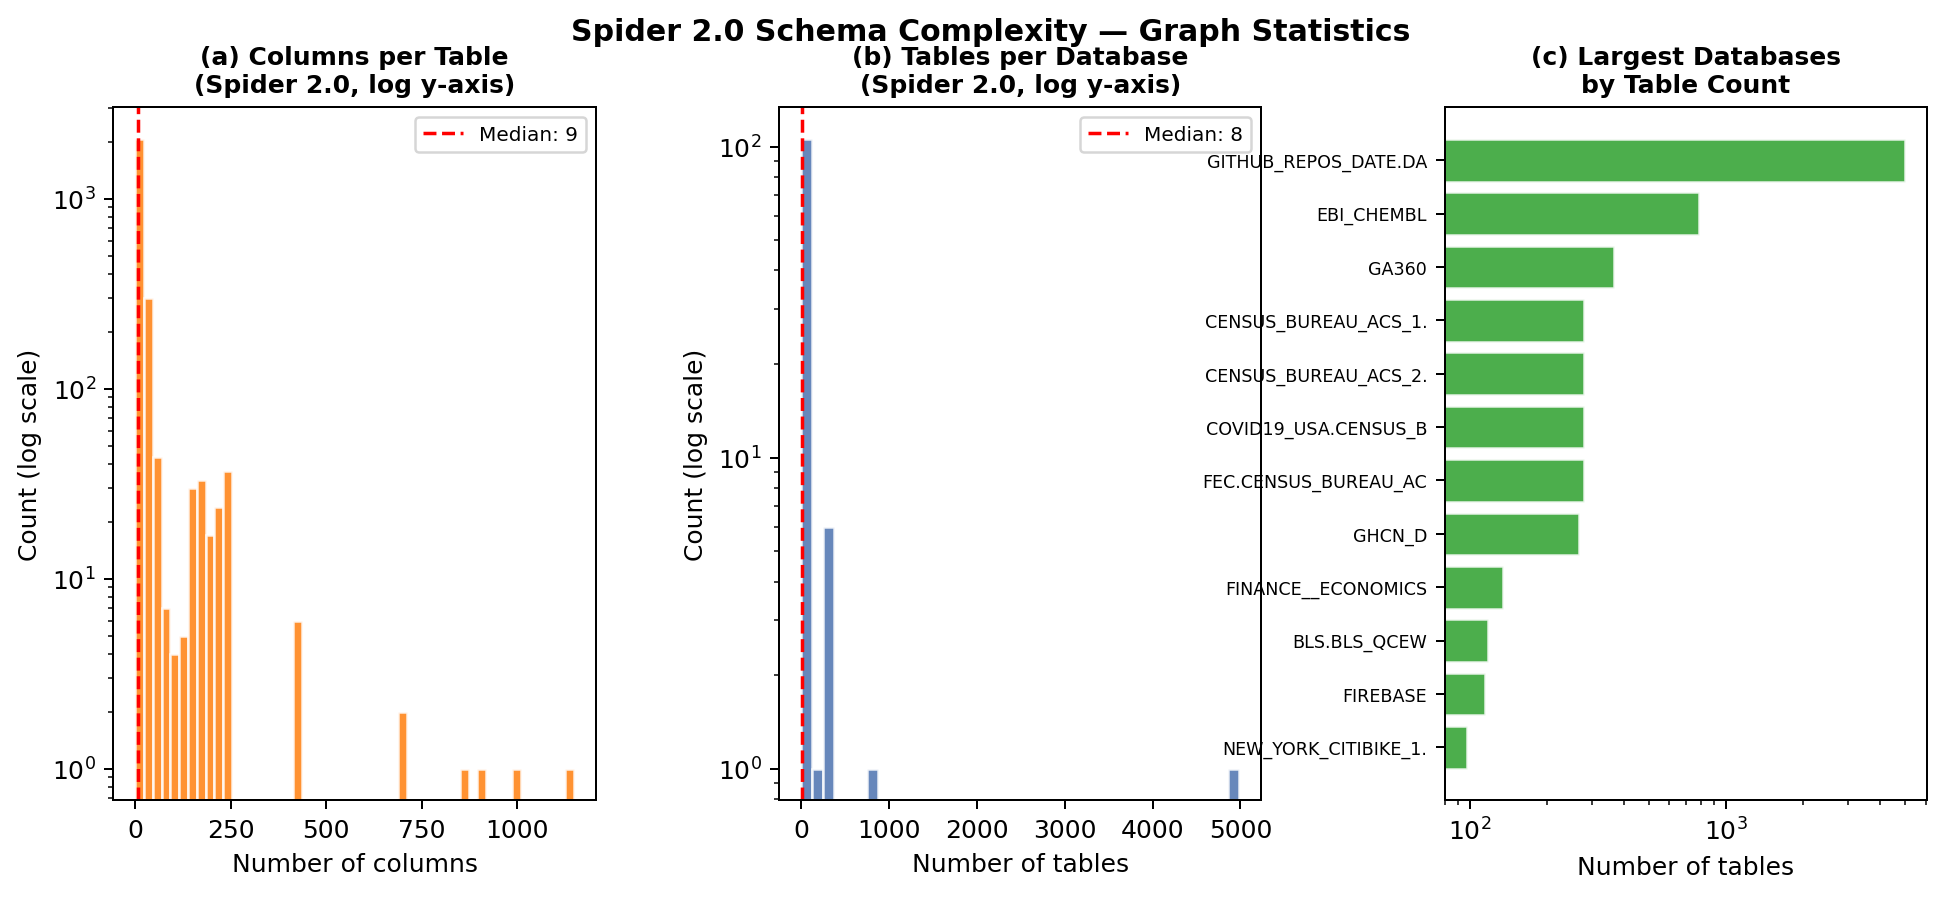
\includegraphics[width=\textwidth]{graph_stats.png}
\caption{Schema complexity distributions for Spider~2.0 databases ingested into Neo4j (ingestion still in progress). Both distributions are heavy-tailed, motivating graph-guided retrieval over flat schema injection. The largest database has 4{,}989 tables---far beyond any LLM context limit.}
\label{fig:graphstats}
\end{figure}

\subsection{Benchmark Baseline (No Results Yet)}

No end-to-end benchmark evaluation of our system has been run yet.
The preliminary results in this section are limited to graph construction and analysis.
The current state-of-the-art on Spider~2.0 is 17--19\% success rate; on BIRD it is approximately 60\% execution accuracy.
Our system will be evaluated against these baselines in the final report, with ablations comparing plain LLM (no graph), text-only RAG, and our full graph-augmented agent.

\subsection{External Knowledge Graph Analysis}

Spider~2.0 ships 69 external knowledge documents---Markdown files containing business logic definitions, domain terminology, and metric formulas that are required to correctly interpret certain questions.
We downloaded and analyzed all 69 documents, finding that 39 of 260 tasks (15.0\%) explicitly reference at least one knowledge document.
These documents exhibit significant length variance (38--6{,}658 words, median 368), reflecting the range from simple column-value glossaries to detailed domain guides.

We model the relationship between databases, documents, and tasks as a bipartite graph $B = (U \cup W, F)$ where $U$ is the set of database nodes, $W$ is the set of document nodes, and an edge $(u, w) \in F$ exists when database $u$ uses document $w$ in at least one task.
This bipartite graph has 28 database nodes, 39 document nodes, and 71 edges.
Figure~\ref{fig:ek} shows the analysis.

Key findings:
\begin{itemize}[leftmargin=*]
  \item \textbf{Knowledge concentration}: a small number of documents are referenced by many tasks. The most referenced document (\texttt{retention\_rate.md}) is used by 4 tasks across multiple databases, indicating that certain business concepts (retention, session definitions) recur across diverse enterprise contexts.
  \item \textbf{Shared knowledge across databases}: some documents are referenced by tasks spanning multiple different databases, creating cross-database edges in the bipartite graph. This motivates storing Metric nodes at the graph level rather than per-database.
  \item \textbf{Identifier density}: across all 69 documents, we extracted 847 unique backtick-quoted identifiers (table/column names, SQL expressions). The most frequently referenced identifiers appear in 3--5 documents, suggesting that certain schema elements are conceptually central across the benchmark.
\end{itemize}

\begin{figure}[h]
\centering
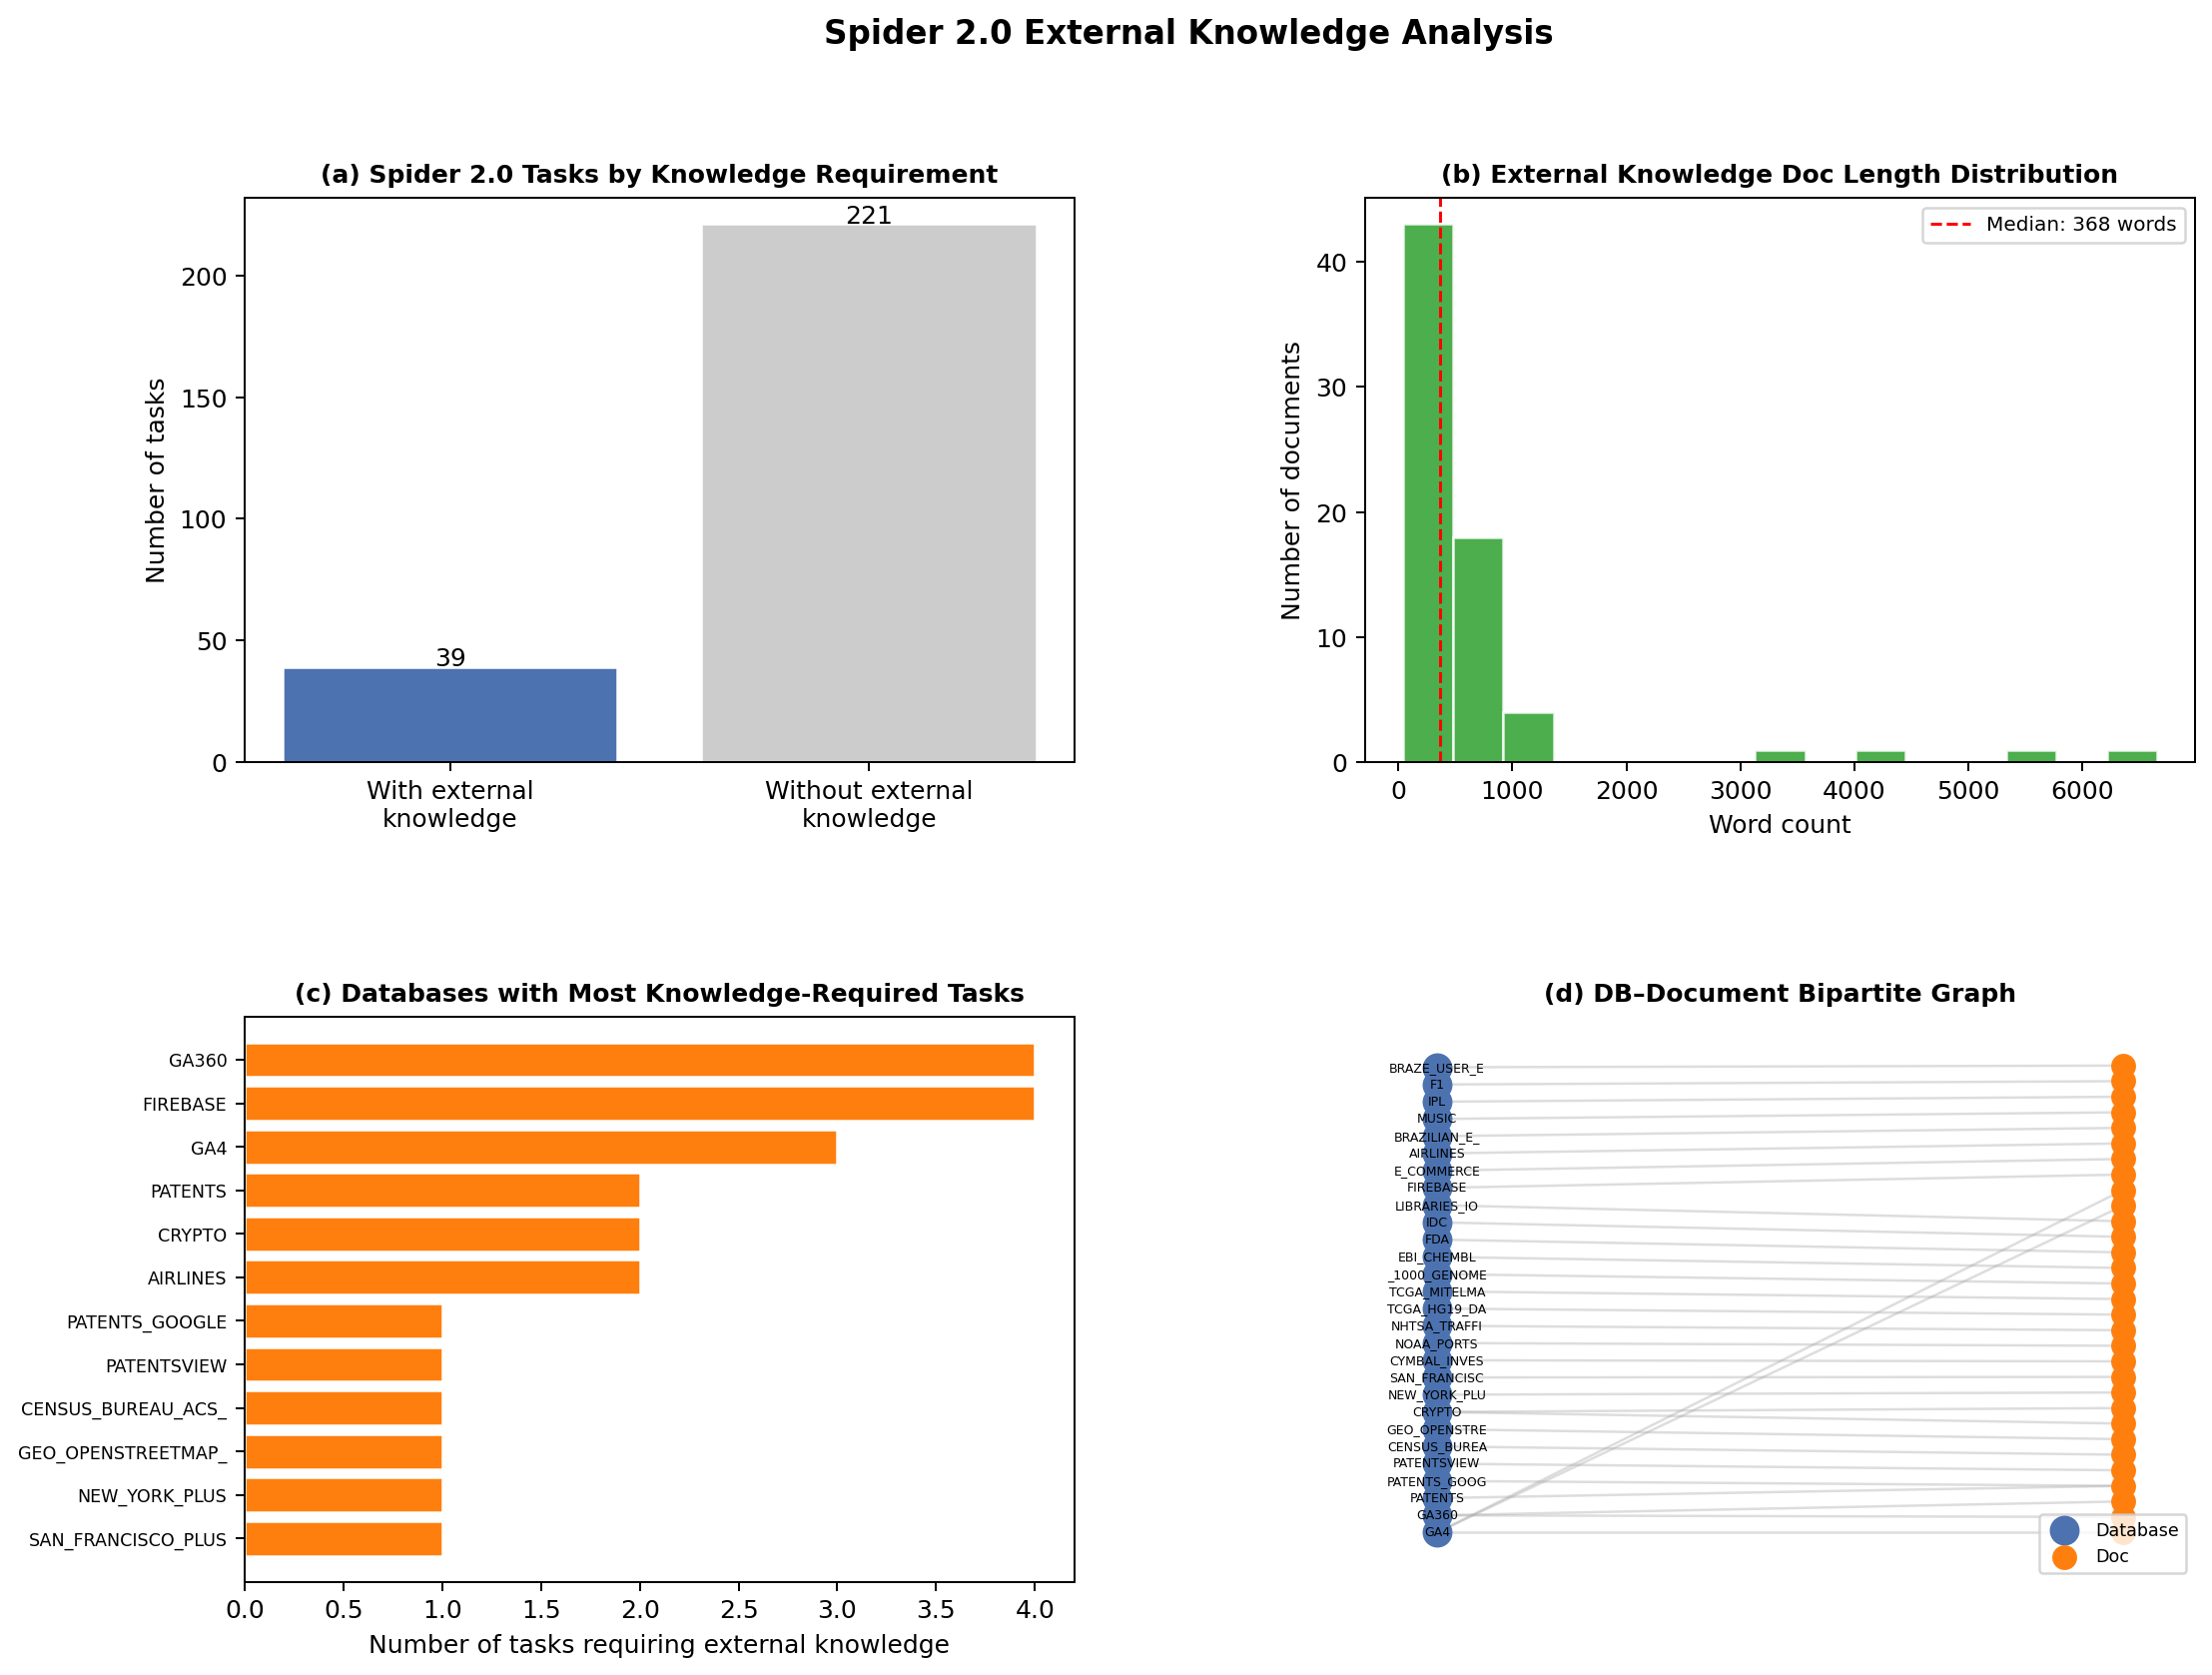
\includegraphics[width=\textwidth]{ek_analysis.png}
\caption{Spider~2.0 external knowledge analysis. (a) Task distribution by knowledge requirement. (b) Document length distribution. (c) Databases with the most knowledge-required tasks. (d) Database--document bipartite graph (blue = database nodes, orange = document nodes).}
\label{fig:ek}
\end{figure}

% -----------------------------------------------------------------------
\section{Complications and Workarounds}
% -----------------------------------------------------------------------

\paragraph{Snowflake MFA authentication.}
The Spider~2.0 Snowflake instance enforces multi-factor authentication.
Key pair authentication (the standard programmatic approach) requires \texttt{ALTER USER} privileges, which the \texttt{PARTICIPANT} role does not have.
Browser-based SSO (\texttt{externalbrowser} authenticator) failed because no SAML identity provider is configured on the account.
We ultimately resolved this by configuring TOTP-based MFA via Microsoft Authenticator and using the \texttt{username\_password\_mfa} Snowflake connector authenticator with session token caching, enabling programmatic access with a single interactive authentication step per session.

\paragraph{Schema query latency.}
Several large Snowflake databases take 5--10 minutes to respond to \texttt{INFORMATION\_SCHEMA.COLUMNS} queries due to the volume of column metadata.
We added per-query timeouts (120 seconds) and a resumable bootstrap design so interrupted runs continue from the last successfully ingested database without data loss.

\paragraph{Missing FK constraints.}
Only 91 FK edges were found across 9{,}093 tables---less than 1 FK per 100 tables.
This is expected for analytical warehouses, which rarely enforce referential integrity at the database level.
We will address this with heuristic column-name matching to infer likely join relationships.

\paragraph{Scope refinement.}
Initial bootstrap code targeted all 155 databases in the Snowflake account.
Upon inspecting the Spider~2.0 task dataset, we found only 114 databases are actually referenced by benchmark tasks.
The bootstrap was updated to filter against the task database list, reducing unnecessary ingestion of irrelevant public datasets.

% -----------------------------------------------------------------------
\section{Work Still To Do}
% -----------------------------------------------------------------------

The remaining tasks in priority order:

\begin{enumerate}[leftmargin=*]
  \item \textbf{Complete Spider~2.0 bootstrap.} Finish ingesting the remaining 23 task databases.
  \item \textbf{Inferred FK edges.} Implement column-name heuristic to create \texttt{:FK \{enforced:false\}} edges across tables in the same database.
  \item \textbf{Sample value ingestion.} For low-cardinality columns, store the top-10 distinct values as \texttt{sample\_values} on Column nodes, preventing the agent from hallucinating invalid filter values.
  \item \textbf{Metric node ingestion.} Parse Spider~2.0 external knowledge Markdown files to populate \texttt{(:Metric)} nodes and link them to columns/tables.
  \item \textbf{Graph tool API implementation.} Implement the six Cypher-backed tools and expose them to the LangGraph agent.
  \item \textbf{Agent implementation.} Wire up the full LangGraph loop with Nemotron NIM for SQL generation and Neo4j for schema retrieval.
  \item \textbf{Baseline runs.} Evaluate a plain LLM baseline (full schema injection) and a text-only RAG baseline on a BIRD subset.
  \item \textbf{Graph-agent evaluation.} Run the graph-augmented agent on the same BIRD subset and measure execution accuracy.
  \item \textbf{Spider~2.0 evaluation.} If time permits, extend evaluation to Spider~2.0 Snowflake tasks.
\end{enumerate}

Tasks 1--4 complete the data and network layer.
Tasks 5--6 implement the agent.
Tasks 7--9 produce the experimental results for the final report.
We consider full Spider~2.0 evaluation (Task 9) a stretch goal contingent on time and available LLM API budget.

\begin{thebibliography}{9}

\bibitem{yu2024spider2}
Fangyu Lei, et al.
\newblock Spider 2.0: Evaluating language agents on real-world enterprise text-to-SQL workflows.
\newblock \emph{ArXiv preprint arXiv:2411.07763}, 2024.

\bibitem{li2024bird}
Jinyang Li, et al.
\newblock Can LLM already serve as a database interface? A big bench for large-scale database grounded text-to-SQL.
\newblock In \emph{NeurIPS}, 2024.

\bibitem{sun2013survey}
Yizhou Sun and Jiawei Han.
\newblock Mining heterogeneous information networks: a structural analysis approach.
\newblock \emph{ACM SIGKDD Explorations Newsletter}, 14(2):20--28, 2013.

\bibitem{yu2018spider}
Tao Yu, et al.
\newblock Spider: A large-scale human-labeled dataset for complex and cross-domain semantic parsing and text-to-SQL task.
\newblock In \emph{EMNLP}, 2018.

\bibitem{gao2023dailsql}
Dawei Gao, et al.
\newblock Text-to-SQL empowered by large language models: A benchmark evaluation.
\newblock \emph{ArXiv preprint arXiv:2308.15363}, 2023.

\bibitem{pourreza2023dinsql}
Mohammadreza Pourreza and Davood Rafiei.
\newblock DIN-SQL: Decomposed in-context learning of text-to-SQL with self-correction.
\newblock In \emph{NeurIPS}, 2023.

\bibitem{fey2023relbench}
Matthias Fey, et al.
\newblock Relational deep learning: Graph representation learning on relational databases.
\newblock \emph{ArXiv preprint arXiv:2312.04615}, 2023.

\bibitem{schlichtkrull2018rgcn}
Michael Schlichtkrull, et al.
\newblock Modeling relational data with graph convolutional networks.
\newblock In \emph{ESWC}, 2018.

\bibitem{langgraph}
LangChain, Inc.
\newblock LangGraph: Build stateful, multi-actor applications with LLMs.
\newblock \url{https://github.com/langchain-ai/langgraph}, 2024.

\end{thebibliography}

\end{document}
